\scanpage{115}
% archive foliation: 114
\figure{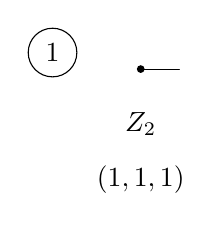
\begin{tikzpicture}[scale=.7,line cap=round]
\node[draw,circle]at(-1.6,.3){$1$};
\begin{scope}[shift={(0.0,0)}]\draw(0,0)--(.7,0);\fill(0,0)circle(2pt);
\node at(0,-1.0){$\uuline{\mathbb Z_2}$};
\node at(0,-2.0){$\left(1,1,1\right)$};
\end{scope}
\end{tikzpicture}}
\figure{\begin{tikzpicture}[scale=.7,line cap=round]
\node[draw,circle]at(-1.6,.3){$2$};
\begin{scope}[shift={(0.0,0)}]\draw(-.7,0)--(.7,0);\fill(0,0)circle(2pt);
\node at(0,-1.0){$\uuline{\mathbb Z_2\times\mathbb Z_2}$};
\node at(0,-2.0){$\left(2,\begin{smallmatrix}1\\1\end{smallmatrix},2\right)$};
\end{scope}
\begin{scope}[shift={(3.1,0)}]\draw(-.5,0)--(.5,0);\fill(-.5,0)circle(2pt);\fill(.5,0)circle(2pt);
\node at(0,-1.0){$\uuline{\mathbb Z_2\times\mathbb Z_2}$};
\node at(0,-2.0){$\left(\begin{smallmatrix}1\\1\end{smallmatrix},2,2\right)$};
\end{scope}
\begin{scope}[shift={(6.2,0)}]\fill(0,0)circle(2pt);\draw(0,0)..controls(1.3,1.4)and(1.4,-1)..(0,0);
\node at(0,-1.0){$\uuline{\mathbb Z_2\times\mathbb Z_2}$};
\node at(0,-2.0){$\left(2,2,\begin{smallmatrix}1\\1\end{smallmatrix}\right)$};
\end{scope}
\draw(3.1,.9)..controls(4.65,.9)and(4.65,.9)..(4.65,1.1)..controls(4.65,.9)and(4.65,.9)..(6.2,.9);
\end{tikzpicture}}
\figure{\begin{tikzpicture}[scale=.7,line cap=round]
\node[draw,circle]at(-1.6,.3){$3$};
\begin{scope}[shift={(0.0,0)}]\fill(0,0)circle(2pt);\draw(0,0)--(90:.65);\draw(0,0)--(210:.65);\draw(0,0)--(330:.65);
\node at(0,-1.0){$\uuline{\mathfrak S_3}$};
\node at(0,-2.0){$\left(3,\begin{smallmatrix}1\\1\\1\end{smallmatrix},3\right)$};
\end{scope}
\begin{scope}[shift={(3.1,0)}]\fill(0,0)circle(2pt);\draw(0,0)..controls(1.3,1.4)and(1.4,-1)..(0,0);\draw(-.8,0)--(0,0);
\node at(0,-1.0){$\mathbb Z_2$};
\node at(0,-2.0){$\left(3,\begin{smallmatrix}2\\1\end{smallmatrix},\begin{smallmatrix}2\\1\end{smallmatrix}\right)$};
\end{scope}
\begin{scope}[shift={(6.2,0)}]\draw(-.7,0)--(.7,0);\fill(-.7,0)circle(2pt);\fill(0,0)circle(2pt);
\node at(0,-1.0){$\mathbb Z_2$};
\node at(0,-2.0){$\left(\begin{smallmatrix}2\\1\end{smallmatrix},\begin{smallmatrix}2\\1\end{smallmatrix},3\right)$};
\end{scope}
\draw(3.1,-1.4)..controls(4.65,-1.4)and(4.65,-1.4)..(4.65,-1.6)..controls(4.65,-1.4)and(4.65,-1.4)..(6.2,-1.4);
\end{tikzpicture}}
\figure{\begin{tikzpicture}[scale=.7,line cap=round]
\node[draw,circle]at(-1.6,.3){$4$};
\begin{scope}[shift={(0.0,0)}]\fill(0,0)circle(2pt);\draw(-.9,0)--(0,0)--(.6,.4);\draw(0,0)--(.6,-.4);\fill(-.9,0)circle(2pt);
\node at(0,-1.0){$\mathbb Z_2$};
\node at(0,-2.0){$\left(\begin{smallmatrix}3\\1\end{smallmatrix},\begin{smallmatrix}2\\1\\1\end{smallmatrix},4\right)$};
\end{scope}
\begin{scope}[shift={(3.1,0)}]\fill(0,0)circle(2pt);\draw(0,0)..controls(1.3,1.4)and(1.4,-1)..(0,0);\draw(-.6,.4)--(0,0)--(-.6,-.4);
\node at(0,-1.0){$\mathbb Z_2$};
\node at(0,-2.0){$\left(4,\begin{smallmatrix}2\\1\\1\end{smallmatrix},\begin{smallmatrix}3\\1\end{smallmatrix}\right)$};
\end{scope}
\begin{scope}[shift={(6.2,0)}]\draw(-1,0)--(1,0);\fill(-.35,0)circle(2pt);\fill(.35,0)circle(2pt);
\node at(0,-1.0){$\mathbb Z_2\times\mathbb Z_2$};
\node at(0,-2.0){$\left(\begin{smallmatrix}2\\2\end{smallmatrix},\begin{smallmatrix}2\\1\\1\end{smallmatrix},4\right)$};
\end{scope}
\begin{scope}[shift={(9.3,0)}]\fill(0,0)circle(2pt);\draw(0,0)..controls(1.3,1.4)and(1.4,-1)..(0,0);\draw(-.7,0)--(.5,0);
\node at(0,-1.0){$\mathbb Z_2\times\mathbb Z_2$};
\node at(0,-2.0){$\left(4,\begin{smallmatrix}2\\1\\1\end{smallmatrix},\begin{smallmatrix}2\\2\end{smallmatrix}\right)$};
\end{scope}
\draw(0.0,-1.4)..controls(1.55,-1.4)and(1.55,-1.4)..(1.55,-1.6)..controls(1.55,-1.4)and(1.55,-1.4)..(3.1,-1.4);
\draw(6.2,-1.4)..controls(7.75,-1.4)and(7.75,-1.4)..(7.75,-1.6)..controls(7.75,-1.4)and(7.75,-1.4)..(9.3,-1.4);
\end{tikzpicture}}
\figure{\begin{tikzpicture}[scale=.7,line cap=round]
\begin{scope}[shift={(0.0,0)}]\fill(0,0)circle(2pt);\draw(0,0)--(90:.65);\draw(0,0)--(180:.65);\draw(0,0)--(270:.65);\draw(0,0)--(0:.65);
\node at(0,-1.0){$\uuline{D_4}$};
\node at(0,-2.0){$\left(4,\begin{smallmatrix}1\\1\\1\\1\end{smallmatrix},4\right)$};
\end{scope}
\begin{scope}[shift={(3.1,0)}]\draw(-1,0)--(1,0);\foreach\x in{-1,0,1}\fill(\x,0)circle(2pt);
\node at(0,-1.0){$\mathbb Z_2\times\mathbb Z_2$};
\node at(0,-2.0){$\left(\begin{smallmatrix}2\\1\\1\end{smallmatrix},\begin{smallmatrix}2\\2\end{smallmatrix},4\right)$};
\end{scope}
\begin{scope}[shift={(6.2,0)}]\fill(0,0)circle(2pt);\draw(0,0)..controls(-1.2,1.3)and(-1.5,-1.2)..(0,0)..controls(1.4,1.2)and(1.4,-1.2)..(0,0);
\node at(0,-1.0){$\mathbb Z_2\times\mathbb Z_2$};
\node at(0,-2.0){$\left(4,\begin{smallmatrix}2\\2\end{smallmatrix},\begin{smallmatrix}2\\1\\1\end{smallmatrix}\right)$};
\end{scope}
\draw(3.1,-1.4)..controls(4.65,-1.4)and(4.65,-1.4)..(4.65,-1.6)..controls(4.65,-1.4)and(4.65,-1.4)..(6.2,-1.4);
\end{tikzpicture}}
\figure{\begin{tikzpicture}[scale=.7,line cap=round]
\begin{scope}[shift={(0.0,0)}]\draw(0,0)ellipse(.5 and.65);\fill(0,.65)circle(2pt);\fill(0,-.65)circle(2pt);
\node at(0,-1.0){$\uuline{D_4}$};
\node at(0,-2.0){$\left(\begin{smallmatrix}2\\2\end{smallmatrix},\begin{smallmatrix}2\\2\end{smallmatrix},\begin{smallmatrix}2\\2\end{smallmatrix}\right)$};
\end{scope}
\begin{scope}[shift={(3.1,0)}]\fill(0,0)circle(2pt);\draw(0,0)..controls(-1.3,1.4)and(-1.4,-1)..(0,0);\draw(0,0)--(.9,0);\fill(.9,0)circle(1pt);
\node at(0,-1.0){$\mathbb Z_2$};
\node at(0,-2.0){$\left(\begin{smallmatrix}3\\1\end{smallmatrix},\begin{smallmatrix}\unsure2\\2\end{smallmatrix},\begin{smallmatrix}1\\3\end{smallmatrix}\right)$};
\end{scope}
\end{tikzpicture}}
\figure{\begin{tikzpicture}[scale=.7,line cap=round]
\node[draw,circle]at(-1.6,.3){$5$};
\begin{scope}[shift={(0.0,0)}]\fill(0,0)circle(2pt);\draw(0,0)--(90:.65);\draw(0,0)--(162:.65);\draw(0,0)--(234:.65);\draw(0,0)--(306:.65);\draw(0,0)--(18:.65);
\node at(0,-1.0){$\uuline{D_5}$};
\node at(0,-2.0){$\left(5\deleted{\unsure{1}},1_5,5\right)$};
\end{scope}
\begin{scope}[shift={(3.1,0)}]\fill(0,0)circle(2pt);\draw(0,0)--(90:.65);\draw(0,0)--(180:.65);\draw(0,0)--(270:.65);\draw(0,0)--(0:.65);\fill(-.65,0)circle(2pt);
\node at(0,-1.0){$\mathbb Z_2$};
\node at(0,-2.0){$\left(\begin{smallmatrix}4\\1\end{smallmatrix},\begin{smallmatrix}2\\1_3\end{smallmatrix},5\right)$};
\end{scope}
\begin{scope}[shift={(6.2,0)}]\fill(0,0)circle(2pt);\draw(0,0)..controls(-1.3,1.4)and(-1.4,-1)..(0,0);\draw(.7,.45)--(0,0)--(.7,0);\draw(0,0)--(.7,-.45);
\node at(0,-1.0){$\mathbb Z_2$};
\node at(0,-2.0){$\left(5,\begin{smallmatrix}2\\1_3\end{smallmatrix},\begin{smallmatrix}4\\1\end{smallmatrix}\right)$};
\end{scope}
\draw(3.1,-1.4)..controls(4.65,-1.4)and(4.65,-1.4)..(4.65,-1.6)..controls(4.65,-1.4)and(4.65,-1.4)..(6.2,-1.4);
\end{tikzpicture}}
\margin{\deleted{$\unsure{\left(\begin{smallmatrix}5\\1_2\end{smallmatrix}\right),}$}}
\figure{\begin{tikzpicture}[scale=.7,line cap=round]
\begin{scope}[shift={(0.0,0)}]\fill(0,0)circle(2pt);\draw(0,0)..controls(-1.3,1.4)and(-1.4,-1)..(0,0);\draw(-.55,0)--(0,0)--(.6,.4);\draw(0,0)--(.6,-.4);
\node at(0,-1.0){$\mathbb Z_2$};
\node at(0,-2.0){$\left(5,\begin{smallmatrix}2\\1_3\end{smallmatrix},\begin{smallmatrix}3\\2\end{smallmatrix}\right)$};
\end{scope}
\begin{scope}[shift={(3.1,0)}]\fill(0,0)circle(2pt);\draw(-.9,0)--(0,0)--(.6,.4);\draw(0,0)--(.6,-.4);\fill(-.5,0)circle(2pt);
\node at(0,-1.0){$\mathbb Z_2$};
\node at(0,-2.0){$\left(\begin{smallmatrix}3\\2\end{smallmatrix},\begin{smallmatrix}2\\1_3\end{smallmatrix},5\right)$};
\end{scope}
\begin{scope}[shift={(6.2,0)}]\fill(0,0)circle(2pt);\draw(0,0)..controls(-1.2,1.3)and(-1.5,-1.2)..(0,0)..controls(1.4,1.2)and(1.4,-1.2)..(0,0);\draw(0,0)--(.4,0);
\node at(0,-1.0){$\mathbb Z_2$};
\node at(0,-2.0){$\left(5,\begin{smallmatrix}2_2\\1\end{smallmatrix},\begin{smallmatrix}\unsure{2_2}\\1\end{smallmatrix}\right)$};
\end{scope}
\begin{scope}[shift={(9.3,0)}]\draw(-1,0)--(1,0);\foreach\x in{-1,-.3,.4}\fill(\x,0)circle(1.5pt);
\node at(0,-1.0){$\mathbb Z_2$};
\node at(0,-2.0){$\left(\begin{smallmatrix}2_2\\1\end{smallmatrix},\begin{smallmatrix}2_2\\1\end{smallmatrix},5\right)$};
\end{scope}
\draw(0.0,-1.4)..controls(1.55,-1.4)and(1.55,-1.4)..(1.55,-1.6)..controls(1.55,-1.4)and(1.55,-1.4)..(3.1,-1.4);
\draw(6.2,-1.4)..controls(7.75,-1.4)and(7.75,-1.4)..(7.75,-1.6)..controls(7.75,-1.4)and(7.75,-1.4)..(9.3,-1.4);
\end{tikzpicture}}
